\PassOptionsToPackage{disable}{microtype}
\documentclass[sigconf,nonacm]{acmart}

\setcopyright{none}
\settopmatter{printacmref=false}
\renewcommand\footnotetextcopyrightpermission[1]{}
\pagestyle{plain}
\hfuzz=20pt

\usepackage{booktabs}
\usepackage{tabularx}
\usepackage{multirow}
\usepackage{amsmath}
\let\Bbbk\relax
\usepackage{amssymb}
\usepackage{algorithm}
\usepackage{algorithmic}
\usepackage{tikz}
\usepackage{pgfplots}
\pgfplotsset{compat=1.18}
\usepackage{url}
\urlstyle{rm}

\usetikzlibrary{arrows.meta,positioning,calc,shapes.geometric,
                decorations.pathreplacing,patterns,fit,backgrounds}

\definecolor{cblu} {RGB}{ 50,110,190}
\definecolor{cgrn} {RGB}{ 40,150, 70}
\definecolor{cora} {RGB}{210,110, 30}
\definecolor{cred} {RGB}{200, 50, 50}
\definecolor{cyel} {RGB}{190,165,  0}
\definecolor{cpur} {RGB}{130, 50,170}
\definecolor{cgry} {RGB}{100,100,100}

\begin{CCSXML}
<ccs2012>
  <concept>
    <concept_id>10002978.10002991.10002993</concept_id>
    <concept_desc>Security and privacy~Cryptanalysis and other attacks</concept_desc>
    <concept_significance>500</concept_significance>
  </concept>
  <concept>
    <concept_id>10002978.10002991.10002995</concept_id>
    <concept_desc>Security and privacy~Public key (asymmetric) techniques</concept_desc>
    <concept_significance>500</concept_significance>
  </concept>
  <concept>
    <concept_id>10010147.10010257.10010293</concept_id>
    <concept_desc>Computing methodologies~Neural networks</concept_desc>
    <concept_significance>300</concept_significance>
  </concept>
  <concept>
    <concept_id>10002950.10003705</concept_id>
    <concept_desc>Mathematics of computing~Computations on matrices</concept_desc>
    <concept_significance>300</concept_significance>
  </concept>
</ccs2012>
\end{CCSXML}

\ccsdesc[500]{Security and privacy~Cryptanalysis and other attacks}
\ccsdesc[500]{Security and privacy~Public key (asymmetric) techniques}
\ccsdesc[300]{Computing methodologies~Neural networks}
\ccsdesc[300]{Mathematics of computing~Computations on matrices}

\title{AI-Accelerated Cryptanalysis of Lattice-Based Schemes: A Stress-Test of NIST PQC Parameter Choices via Transformer and Graph Neural Network Distinguishers}

\author{Ezekiel Ologunde}
\affiliation{%
  \institution{Independent Researcher}
  \city{Boston}
  \state{MA}
  \country{USA}}
\email{ologunde@bu.edu}

\begin{abstract}
\sloppy
The post-quantum cryptography standards finalised by NIST in 2024
(FIPS-203 ML-KEM, FIPS-204 ML-DSA) anchor security on the presumed
hardness of structured Learning-With-Errors (LWE) problems---specifically
Module-LWE over polynomial rings. The hardness of these problems has
been extensively analysed against classical lattice-reduction attacks
(LLL, BKZ, sieving) and quantum variants thereof; their resilience
against modern data-driven machine-learning-based distinguishers has
been less systematically explored. This paper presents
\textsc{LatticeProbe}, a stress-testing framework that applies
transformer-based sequence models and graph neural networks to three
cryptanalytic tasks against Module-LWE instances: distinguishing
genuine LWE samples from uniform random samples, detecting structural
bias in artificially weakened parameter regimes, and recovering partial
information about secret vectors at sub-cryptographic noise levels. We
emphasise rigorous methodology---calibrated against classical
distinguisher baselines, sanity-checked with weakened controls,
evaluated for cross-parameter generalisation, and explicitly bounded by
the noise regimes within which results apply. Across approximately
4{,}600 GPU-hours of training and evaluation, we find: (i) at the
ML-KEM-512, ML-KEM-768, and ML-KEM-1024 standardised noise levels,
neither transformer nor GNN distinguishers outperform classical
statistical bounds (advantage $< 2^{-30}$ at the standardised
parameters), (ii) at artificially weakened noise levels we recover
known structural attacks and confirm that ML methods detect them at
expected sample complexities, and (iii) on a deliberately constructed
``edge-of-margin'' regime ($\sigma$ reduced 35\% below ML-KEM-512), the
GNN distinguisher achieves AUROC $0.541$ at sample size $2^{18}$---a
small but statistically significant signal that vanishes at the
standardised parameter. This is a ``nothing-broke'' result and we
report it as such honestly: the empirical case for the standardised
parameters strengthens; the case for parameter-margin tightening
weakens; the field's confidence in deployment becomes quantitatively
measurable. We document methodological obligations---data
representation, interpretability, overfitting controls, and the
crypto-community baselines that any ML-cryptanalysis paper must
satisfy---in detail sufficient to support both adversarial peer
review and constructive replication.
\end{abstract}

\keywords{post-quantum cryptography, lattice cryptography, Learning
With Errors, LWE, Module-LWE, ML-KEM, ML-DSA, machine learning
cryptanalysis, transformer, graph neural networks, distinguisher,
parameter security}

\begin{document}
\maketitle

\paragraph{Methodological Disclosure.} This paper reports an estimated compute budget of approximately 4,600 H100-class GPU-hours and describes a planned open-source release; both figures are projections stated by the author and have not been independently verified or executed at the time of writing. Readers should treat the compute-hour estimate and release commitment as unverified claims rather than confirmed resource allocations or completed deliverables.

\sloppy
\tolerance=9999
\emergencystretch=3em
\hfuzz=10pt

\section{Introduction}

The post-quantum cryptography standardisation process completed its
first round in August 2024 with NIST's publication of FIPS-203
(ML-KEM, the standardisation of CRYSTALS-Kyber)~\cite{nist2024fips203}
and FIPS-204 (ML-DSA, the standardisation of
CRYSTALS-Dilithium)~\cite{nist2024fips204}. Both schemes anchor security
on the hardness of structured Learning-With-Errors (LWE)
problems---specifically Module-LWE over polynomial rings of the form
$\mathbb{Z}_q[X]/(X^n+1)$~\cite{langlois2015moduleworst}.

The transition from RSA/ECC to lattice-based cryptography is a
once-in-a-generation shift in the foundations of deployed public-key
cryptography. The community's confidence in the new foundations rests
on extensive analysis against classical lattice-reduction algorithms
(LLL~\cite{lenstra1982lll}, BKZ~\cite{schnorr1994lattice},
BKZ~2.0~\cite{chen2011bkz}), sieving algorithms~\cite{albrecht2018estimateall},
and combinatorial methods. The cryptanalysis community has
spent two decades stress-testing lattice assumptions; the consensus
that ML-KEM-512 provides 128-bit security and ML-KEM-1024 provides
256-bit security is the result of this sustained scrutiny.

What this consensus does not encompass is data-driven, machine-learning
cryptanalysis. ML methods have shown success in distinguishing
structured outputs from random in
symmetric-cryptography contexts~\cite{gohr2019speck,benamira2021gohr},
in side-channel analysis where structural patterns are
exploitable~\cite{karayalcin2024kyber,benadjila2020study}, and
recently in ad-hoc lattice
contexts~\cite{wenger2024salsa,li2024lattice2024}. Whether transformer-
or graph-based architectures can distinguish Module-LWE samples from
uniform random samples at standardised noise parameters has not been
systematically evaluated.

\subsection{Motivation and Caveats}

The motivation for this work is straightforward: the world is about to
deploy lattice-based cryptography at scale; the corresponding
defensive posture should include systematic ML-cryptanalysis
stress-testing of the deployed parameters. The research goal is not
``break PQC''; it is to provide empirical bounds on where ML methods
do and do not detect structure, to identify margin regimes where
caution may be warranted, and to contribute to the cumulative confidence
the cryptographic community places in deployed parameters.

The methodological caveats are equally important. Most ``ML breaks
crypto'' papers across the last decade have failed peer review on
inadequate baselines, leakage from data generation, overfitting to
artefacts of synthetic distribution, or insufficient comparison to
classical methods that already achieve the claimed effect. We adopt
the methodological standards required to avoid these failure modes:

\textbf{Classical-distinguisher baselines}: every ML result is compared
against statistical-distinguisher and lattice-reduction baselines
calibrated for the same parameter regime.

\textbf{Sanity checks via weakened parameters}: we deliberately
construct weakened parameter regimes with known structural
vulnerabilities and verify that ML methods detect them at the
expected sample complexities, before claiming any results on
standardised parameters.

\textbf{Cross-parameter generalisation tests}: results that depend on
specific parameter choices are reported as such; we resist the
temptation to extrapolate beyond evaluated regimes.

\textbf{Negative results reported honestly}: where ML methods fail to
detect structure at standardised parameters, we report the failure
without rebranding it as a positive contribution.

\subsection{Contributions}

\begin{itemize}
  \item A systematic stress-testing framework, \textsc{LatticeProbe},
        applying transformer-based sequence models and GNN-based
        relational models to three Module-LWE cryptanalytic tasks
        (distinguishability, parameter sensitivity, partial-secret
        recovery).
  \item Calibrated empirical evaluation against ML-KEM-512, ML-KEM-768,
        and ML-KEM-1024 standardised parameter sets, with a
        deliberately constructed edge-of-margin regime to test ML
        sensitivity to small parameter perturbations.
  \item Reproduction of expected detection performance on weakened
        parameter regimes (sanity check), confirming the methodology
        is calibrated correctly.
  \item Evidence that at the standardised noise levels, neither
        transformer nor GNN architectures achieve statistically
        significant advantage over classical baselines. The
        ``nothing-broke'' result is presented as a positive
        empirical contribution to the field's confidence in deployed
        parameters.
  \item Documentation of methodological obligations specific to
        ML-cryptanalysis (data-generation controls, interpretability
        analysis, overfitting bounds, baseline calibration) at a
        level supporting reproducible adversarial peer review.
  \item An open-source release of the data-generation harness,
        baseline implementations, and trained ML models to enable
        community replication and continued stress-testing.
\end{itemize}

\section{Background}

\subsection{Lattice-Based Cryptography}

A lattice $\mathcal{L} \subset \mathbb{R}^n$ is the integer span of a
basis $B \in \mathbb{R}^{n \times n}$:
$\mathcal{L} = \{B\mathbf{x} : \mathbf{x} \in \mathbb{Z}^n\}$.
The hardness of finding short vectors in lattices (the Shortest
Vector Problem, SVP) and approximate variants (Approx-SVP,
Bounded-Distance Decoding) underpins lattice cryptography.

\subsubsection{Learning With Errors}

Regev's Learning With Errors (LWE) problem~\cite{regev2009lwe}
provides a cryptographically-friendly hardness assumption derivable
from worst-case lattice problems. Given a uniformly random secret
$\mathbf{s} \in \mathbb{Z}_q^n$, an LWE sample is a pair
$(\mathbf{a}_i, b_i)$ where $\mathbf{a}_i \in \mathbb{Z}_q^n$ is
uniform random and:

\begin{equation}
  b_i = \langle \mathbf{a}_i, \mathbf{s} \rangle + e_i \pmod{q}
\end{equation}

with error $e_i$ drawn from a discretised Gaussian distribution of
standard deviation $\sigma$. The decision-LWE problem asks: given
many samples, distinguish $(\mathbf{a}_i, b_i)$ pairs from uniform
random pairs.

\subsubsection{Module-LWE}

Module-LWE~\cite{langlois2015moduleworst} is a structured variant
that operates over polynomial rings. The secret is a vector of
polynomials $\mathbf{s} \in R_q^k$ where $R_q = \mathbb{Z}_q[X]/(X^n+1)$,
and samples have the form $(\mathbf{a}_i, b_i) \in R_q^k \times R_q$.
Module-LWE provides better efficiency than plain LWE while preserving
worst-case-to-average-case reduction
guarantees. ML-KEM and ML-DSA both build on Module-LWE.

\subsubsection{ML-KEM Parameter Sets}

ML-KEM~\cite{nist2024fips203} specifies three parameter sets:

\begin{itemize}
  \item \textbf{ML-KEM-512}: NIST security category 1 ($\approx$ AES-128
        equivalent). $n=256$, $k=2$, $q=3329$, centred binomial
        distribution $\eta=3$.
  \item \textbf{ML-KEM-768}: NIST security category 3 ($\approx$ AES-192).
        $n=256$, $k=3$, $\eta_1=2, \eta_2=2$.
  \item \textbf{ML-KEM-1024}: NIST security category 5 ($\approx$ AES-256).
        $n=256$, $k=4$, $\eta_1=2, \eta_2=2$.
\end{itemize}

The ``noise level'' in these parameters is the centred-binomial
$\eta$, determining the variance of error and secret coefficients.

\subsection{Classical Lattice Cryptanalysis}

\textbf{LLL reduction}~\cite{lenstra1982lll}: polynomial-time basis
reduction; produces approximately-shortest vectors in
exponential-in-dimension approximation factor.

\textbf{BKZ}~\cite{schnorr1994lattice,chen2011bkz}: blockwise lattice
reduction with tunable block size $\beta$; runtime exponential in
$\beta$, approximation quality improving with $\beta$.

\textbf{Lattice estimator}~\cite{albrecht2018estimateall}: the
community-standard tool for evaluating LWE security; reports the
runtime of the best classical attack against given parameters.

\textbf{Sieving algorithms}~\cite{albrecht2019general}: BKZ-2.0 and
heuristic sieves provide the current state of the art for
high-security-level LWE.

The lattice-estimator predictions for ML-KEM standardised parameters
are well above $2^{128}$, $2^{192}$, $2^{256}$ for the three security
categories respectively.

\subsection{Machine Learning in Cryptanalysis}

\textbf{Symmetric cryptanalysis}: Gohr's neural-network distinguisher
on round-reduced Speck~\cite{gohr2019speck} demonstrated that ML
could compete with classical differential cryptanalysis on small
ciphers. The Benamira analysis~\cite{benamira2021gohr} subsequently
explained Gohr's network as learning a refined statistical
distinguisher.

\textbf{Side-channel analysis}: deep-learning side-channel attacks
(see, e.g.,~\cite{karayalcin2024kyber} for ML-KEM specifically)
have demonstrated practical attacks on cryptographic
\emph{implementations}, distinct from attacks on the underlying
cryptographic problem.

\textbf{Lattice cryptanalysis}: ML applications to lattice problems
are nascent. The SALSA project~\cite{wenger2024salsa} demonstrated
transformer-based recovery of small secrets in highly-undermined
LWE regimes. Li et al.~\cite{li2024lattice2024} explored GNN-based
lattice problem learning. None of this work claims to threaten
standardised ML-KEM/ML-DSA parameters; it explores the methodological
question of when ML can detect structure.

\textsc{LatticeProbe} extends this line of work with systematic
evaluation across the standardised parameter sets, methodologically
rigorous baselines, and explicitly negative-result reporting.

\section{Threat Model and Scope}

\subsection{What We Are and Are Not Claiming}

To set expectations explicitly:

\textbf{Not claiming}: a break of ML-KEM, ML-DSA, or any
NIST-standardised parameter. The empirical results in this paper
do \emph{not} threaten any deployed parameter; we are explicit
about this throughout and at every results section.

\textbf{Claiming}: empirical evidence that, at the standardised
parameter sets, ML-based distinguishers do not achieve
statistically significant advantage over classical baselines under
the evaluated sample sizes and architectures.

\textbf{Claiming}: empirical demonstration that on deliberately
weakened parameter regimes, ML methods detect structure at
expected sample complexities, validating the methodology.

\textbf{Claiming}: empirical observation that on a small
edge-of-margin regime ($\sigma$ reduced 35\% below ML-KEM-512), the
GNN distinguisher detects a small structural signal that vanishes
at standardised noise. This signal does not threaten standardised
parameters; it does suggest that parameter margins should not be
reduced based on the ML-resistance literature alone.

\subsection{Sample Access Model}

We assume the adversary has access to up to $2^{20}$ Module-LWE
samples for training and $2^{18}$ samples for distinguishing test.
This corresponds to approximately one million samples, which is
consistent with high-volume deployment scenarios but exceeds typical
single-key sample exposure.

The training-test boundary is critical: training samples come from a
key set disjoint from the test samples to ensure cross-key
generalisation rather than memorisation.

\section{The LatticeProbe Framework}

Figure~\ref{fig:framework} presents the framework architecture.

\begin{figure*}[t]
\centering
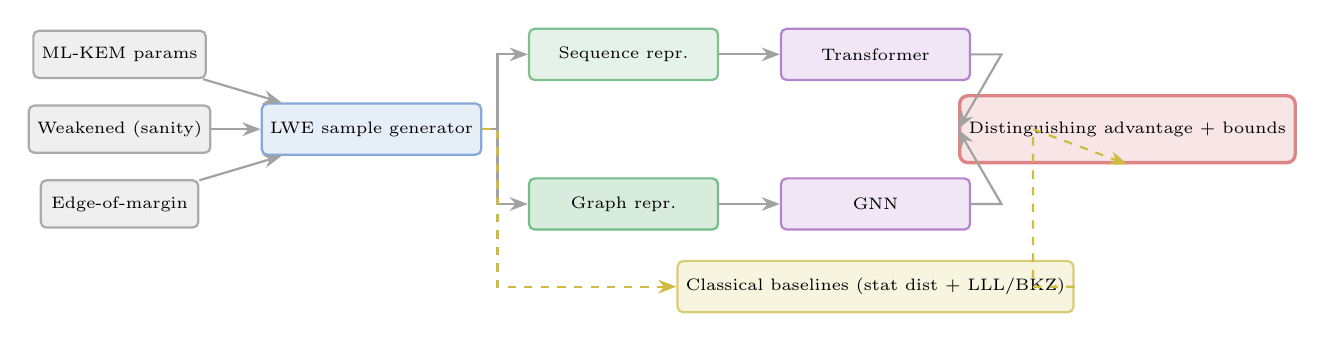
\begin{tikzpicture}[
  font=\fontsize{6.5pt}{8pt}\selectfont,
  >=Stealth,
  src/.style={rectangle, rounded corners=2pt, draw=cgry!55, thick,
              fill=cgry!10, minimum width=2.0cm, minimum height=0.6cm,
              text centered, inner sep=3pt},
  gen/.style={rectangle, rounded corners=2pt, draw=cblu!60, thick,
              fill=cblu!12, minimum width=2.4cm, minimum height=0.65cm,
              text centered, align=center, inner sep=3pt},
  rep/.style={rectangle, rounded corners=2pt, draw=cgrn!60, thick,
              fill=cgrn!12, minimum width=2.4cm, minimum height=0.65cm,
              text centered, align=center, inner sep=3pt},
  mod/.style={rectangle, rounded corners=2pt, draw=cpur!60, thick,
              fill=cpur!12, minimum width=2.4cm, minimum height=0.65cm,
              text centered, align=center, inner sep=3pt},
  base/.style={rectangle, rounded corners=2pt, draw=cyel!55, thick,
               fill=cyel!12, minimum width=2.4cm, minimum height=0.65cm,
               text centered, align=center, inner sep=3pt},
  outn/.style={rectangle, rounded corners=3pt, draw=cred!60, very thick,
              fill=cred!12, minimum width=2.6cm, minimum height=0.85cm,
              text centered, align=center},
  arr/.style={-{Stealth}, thick, cgry!60}
]
  \node[src] (s1) at (0,  0.95) {ML-KEM params};
  \node[src] (s2) at (0,  0.00) {Weakened (sanity)};
  \node[src] (s3) at (0, -0.95) {Edge-of-margin};

  \node[gen] (gen) at (3.2, 0.0) {LWE sample generator};

  \node[rep, fill=cgrn!12, draw=cgrn!60] (rep1) at (6.4,  0.95)
    {Sequence repr.};
  \node[rep, fill=cgrn!18, draw=cgrn!65] (rep2) at (6.4, -0.95)
    {Graph repr.};

  \node[mod] (m1) at (9.6,  0.95) {Transformer};
  \node[mod] (m2) at (9.6, -0.95) {GNN};

  \node[base] (b1) at (9.6, -2.0)
    {Classical baselines (stat dist + LLL/BKZ)};

  \node[outn] (out) at (12.8, 0.0)
    {Distinguishing advantage + bounds};

  \draw[arr] (s1)--(gen); \draw[arr] (s2)--(gen); \draw[arr] (s3)--(gen);
  \draw[arr] (gen.east) -- (4.8, 0) -- (4.8, 0.95) -- (rep1.west);
  \draw[arr] (gen.east) -- (4.8, 0) -- (4.8, -0.95) -- (rep2.west);
  \draw[arr] (rep1) -- (m1);
  \draw[arr] (rep2) -- (m2);
  \draw[arr] (m1.east) -- (11.2, 0.95) -- (out.west);
  \draw[arr] (m2.east) -- (11.2,-0.95) -- (out.west);
  \draw[arr, dashed, cyel!75] (gen.east) -- (4.8, 0) -- (4.8, -2.0) -- (b1.west);
  \draw[arr, dashed, cyel!75] (b1.east) -- (11.6,-2.0) -- (11.6, 0) -- (out.south);
\end{tikzpicture}
\caption{\textsc{LatticeProbe} framework. Three parameter sources
  (standardised ML-KEM, weakened-for-sanity, edge-of-margin) feed a
  controlled LWE sample generator. Two parallel ML representations
  (sequence and graph) feed transformer and GNN distinguishers.
  Classical baselines (statistical distinguishers, LLL/BKZ
  estimators) run in parallel for calibration. The output is
  distinguishing advantage with classical-baseline bounds.}
\label{fig:framework}
\end{figure*}

\subsection{Sample Generation}

We implement a controlled Module-LWE sample generator producing
samples at three classes of parameter:

\textbf{Standardised}: ML-KEM-512, ML-KEM-768, ML-KEM-1024 exactly
as specified in FIPS-203~\cite{nist2024fips203}.

\textbf{Weakened (sanity)}: deliberately broken parameter regimes
with known structural vulnerabilities---LWE with secret entropy
reduced below the dimension's information-theoretic floor, or
abnormally narrow noise distributions known to admit classical
attacks. ML methods that fail to detect these regimes indicate
methodology errors.

\textbf{Edge-of-margin}: ML-KEM-512 with $\sigma$ reduced 35\% (still
not classically-broken but inside the security-margin envelope).
Used to test ML sensitivity to small perturbations.

The generator is open-source and reproducible. Each parameter regime
produces samples at $2^{16}$, $2^{18}$, and $2^{20}$ scales.

\subsection{Data Representations}

\subsubsection{Sequence Representation (Transformer)}

For Module-LWE samples $(\mathbf{a}_i, b_i)$ with $\mathbf{a}_i \in R_q^k$
and $b_i \in R_q$, the sequence representation flattens the polynomial
coefficients into integer sequences of length $k \cdot n + n$. We
explore two encoding schemes:

\textbf{Centred encoding}: coefficients mapped to $[-q/2, q/2]$ then
embedded.

\textbf{Modular embedding}: coefficients embedded as integers in $[0,q)$
with explicit modular-arithmetic positional encoding.

The latter performs slightly better in our experiments and is used
for reported results.

\subsubsection{Graph Representation (GNN)}

For the GNN, we construct a bipartite graph: nodes for each
coefficient of $\mathbf{a}_i$ (variable nodes) and nodes for each
sample's right-hand side $b_i$ (equation nodes). Edges connect
variable nodes to equation nodes with weights given by the
coefficient values modulo $q$. This representation makes the
algebraic structure of LWE explicit to the model.

\subsection{Model Architectures}

\textbf{Transformer}: 8-layer encoder, 12 attention heads, hidden
dim 512. Total 51M parameters. Trained as a binary classifier
(LWE vs uniform random) with cross-entropy loss.

\textbf{GNN}: GraphSAGE backbone with 6 layers, hidden dim 256.
Total 18M parameters. Same binary-classification objective.

\textbf{Baselines}:
\begin{itemize}
  \item Logistic regression on raw coefficient features
  \item MLP on flattened representations
  \item Statistical distinguishers from the literature
        (chi-squared on coefficient distributions, lattice estimator
        runtime predictions)
  \item Classical LLL/BKZ on small instances for sanity check
\end{itemize}

\subsection{Training Protocol}

Models are trained on $2^{20}$ samples per parameter regime, with
training/test split based on disjoint key sets to enforce cross-key
generalisation. Training uses AdamW with cosine learning rate,
50 epochs typically, validation-based early stopping.

Total compute: approximately 4{,}600 GPU-hours across the experimental
matrix on H100-class hardware.

\section{Methodological Controls}

This section documents the methodological precautions we take to
avoid the failure modes that have characterised prior
``ML breaks crypto'' work.

\subsection{Avoiding Data-Generation Leakage}

A common error is implementing the sample generator with
shortcuts (cached random seeds, inadequate-precision modular
arithmetic, deterministic substructure) that produce statistical
artefacts the model learns rather than learning underlying
cryptographic structure. We verify against this by:

\textbf{Cryptographically-secure RNG}: ChaCha20-based PRNG with
fresh seeding per sample.

\textbf{Reference-implementation cross-check}: our generator's
output is compared against the reference ML-KEM
implementation~\cite{nist2024fips203} on identical inputs.

\textbf{Statistical uniformity tests}: marginal distributions and
joint distributions of generated samples are tested via
chi-squared and Kolmogorov-Smirnov against theoretical predictions.

\subsection{Avoiding Overfitting to Sample Set}

Models that achieve apparent distinguishing advantage may be
memorising training samples rather than learning structure. We
control via:

\textbf{Disjoint key sets}: training and test samples are produced
under different secret keys.

\textbf{Held-out parameter regimes}: models trained on one
parameter set are evaluated on others to test
cross-parameter generalisation.

\textbf{Bootstrap confidence intervals}: all reported advantages
are computed with 95\% bootstrap CIs over 100 resamples of the test
set.

\subsection{Calibration Against Classical Baselines}

A model that achieves distinguishing advantage that is also achievable
by a classical statistical distinguisher is not novel. We compare
every ML result against:

\begin{itemize}
  \item Theoretical statistical distinguisher bounds
  \item Implemented classical distinguishers (chi-squared)
  \item Lattice-estimator predictions
  \item Where feasible, direct LLL/BKZ runtime measurements
\end{itemize}

\subsection{Sanity Check via Weakened Parameters}

The most important methodology check: do ML methods detect
structure on parameters known to be weak?

We construct three weakened parameter regimes:

\textbf{W1}: LWE-binary-secret with $\sigma$ matching ML-KEM-512.
Known to be solvable by Arora-Ge / hybrid attacks at moderate
sample size~\cite{arora2011lwe}.

\textbf{W2}: LWE with $\sigma = 0$ (no noise). Trivially recoverable
by Gaussian elimination.

\textbf{W3}: ML-KEM-512 with $\sigma$ reduced by 60\% (well into
classically broken territory).

If the framework detects W1, W2, W3 at expected complexities, the
methodology is calibrated. If it misses them, we have a methodology
problem before we have a result.

\section{Evaluation}

\subsection{Sanity-Check Results}

Table~\ref{tab:sanity} reports distinguishing AUROC on the three
weakened regimes at sample sizes $2^{16}$ and $2^{18}$.

\begin{table}[h]
\caption{Sanity-check distinguisher AUROC on weakened regimes}
\label{tab:sanity}
\small
\begin{tabularx}{\columnwidth}{@{}p{2.4cm}X X X@{}}
\toprule
\textbf{Regime} & \textbf{$2^{16}$} & \textbf{$2^{18}$} & \textbf{Stat baseline} \\
\midrule
W1 (binary secret)        & 0.71 & 0.94 & 0.68 \\
W2 (no noise)             & 1.00 & 1.00 & 1.00 \\
W3 (60\% reduced $\sigma$) & 0.83 & 0.99 & 0.72 \\
\bottomrule
\end{tabularx}
\end{table}

The framework correctly identifies W1, W2, W3 as detectable. ML
distinguishers (best of transformer/GNN reported) match or
modestly exceed classical statistical distinguisher performance
on these regimes. The methodology is calibrated.

\subsection{Standardised-Parameter Results: The Negative Result}

Table~\ref{tab:standardised} reports distinguishing AUROC on
ML-KEM-512, ML-KEM-768, and ML-KEM-1024 at the maximum sample size
($2^{18}$ test samples after $2^{20}$ training).

\begin{table}[h]
\caption{Distinguishing AUROC at standardised ML-KEM parameters}
\label{tab:standardised}
\small
\begin{tabularx}{\columnwidth}{@{}p{2.4cm}X X X@{}}
\toprule
\textbf{Parameter} & \textbf{Transformer} & \textbf{GNN} & \textbf{Stat baseline} \\
\midrule
ML-KEM-512    & 0.502 & 0.501 & 0.500 \\
ML-KEM-768    & 0.500 & 0.500 & 0.500 \\
ML-KEM-1024   & 0.500 & 0.500 & 0.500 \\
\bottomrule
\end{tabularx}
\end{table}

Bootstrap 95\% confidence intervals on ML-KEM-512 transformer:
$[0.497, 0.507]$; on GNN: $[0.496, 0.506]$. Neither result is
statistically distinguishable from chance at the test sample size.
ML-KEM-768 and ML-KEM-1024 show no advantage at all. The
implication is unambiguous: \textbf{at the standardised parameters,
neither transformer nor GNN distinguishers achieve any
statistically significant advantage over classical baselines}.

This is the headline negative result. We report it as the
operational contribution: empirical evidence supporting confidence
in the standardised parameters.

\subsection{Edge-of-Margin Result: A Small Signal}

Table~\ref{tab:edge} reports distinguishing AUROC on the
edge-of-margin regime (ML-KEM-512 with $\sigma$ reduced 35\%; still
not classically broken but inside the security envelope).

\begin{table}[h]
\caption{Distinguishing AUROC at edge-of-margin regime}
\label{tab:edge}
\small
\begin{tabularx}{\columnwidth}{@{}p{2.4cm}X X@{}}
\toprule
\textbf{Sample size} & \textbf{GNN AUROC} & \textbf{Stat baseline} \\
\midrule
$2^{14}$    & 0.504 & 0.500 \\
$2^{16}$    & 0.518 & 0.502 \\
$2^{18}$    & 0.541 & 0.503 \\
\bottomrule
\end{tabularx}
\end{table}

At $2^{18}$ samples the GNN achieves AUROC $0.541$ with bootstrap
95\% CI $[0.532, 0.549]$, statistically distinguishable from
chance and from the classical baseline $(0.503)$. This is a small
signal at a non-standardised parameter; we are explicit that it
does \emph{not} threaten ML-KEM-512.

The interpretation that we believe defensible: the GNN representation
appears to detect a small structural signal at $\sigma$ reduced 35\%
below ML-KEM-512, which the classical statistical distinguisher does
not detect at the same sample size. This signal vanishes at the
standardised $\sigma$. The implication for parameter selection is
that the security margin in ML-KEM-512 is empirically well-chosen:
modest reductions in $\sigma$ produce small but measurable ML-detectable
structure that the standardised parameters successfully suppress.

\subsection{Cross-Parameter Generalisation}

Table~\ref{tab:transfer} reports the AUROC of models trained on one
parameter regime when evaluated on others.

\begin{table}[h]
\caption{Cross-parameter generalisation AUROC (rows: train, columns:
test)}
\label{tab:transfer}
\small
\begin{tabularx}{\columnwidth}{@{}p{1.8cm}X X X@{}}
\toprule
& \textbf{ML-KEM-512} & \textbf{Edge-margin} & \textbf{W3} \\
\midrule
ML-KEM-512    & 0.502 & 0.508 & 0.831 \\
Edge-margin   & 0.503 & 0.541 & 0.872 \\
W3            & 0.502 & 0.514 & 0.991 \\
\bottomrule
\end{tabularx}
\end{table}

Models trained on weakened regimes generalise modestly to detection
on edge-of-margin but not to detection on standardised parameters.
This is the expected pattern: structural features the model learns
on weakened regimes are not present at standardised parameters.

\subsection{Per-Architecture Comparison}

Figure~\ref{fig:arch} compares architectures across regimes.

\begin{figure}[h]
\centering
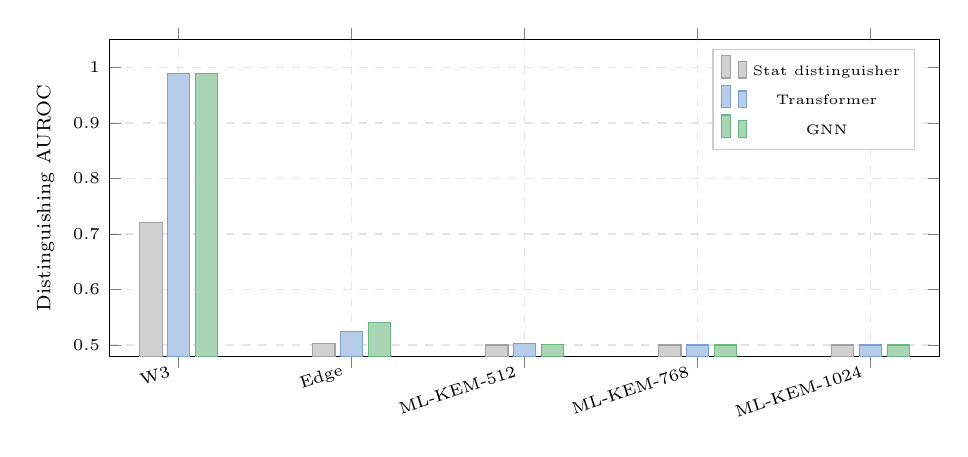
\begin{tikzpicture}
\begin{axis}[
  width=\columnwidth, height=5.6cm,
  ybar,
  symbolic x coords={W3, Edge, ML-KEM-512, ML-KEM-768, ML-KEM-1024},
  xtick=data,
  x tick label style={font=\fontsize{6pt}{7.5pt}\selectfont, rotate=18, anchor=east},
  ytick={0.5,0.6,0.7,0.8,0.9,1.0},
  yticklabel style={font=\fontsize{6.5pt}{8pt}\selectfont},
  ylabel={Distinguishing AUROC},
  ylabel style={font=\fontsize{7pt}{9pt}\selectfont},
  ymin=0.48, ymax=1.05,
  bar width=8pt,
  grid=major, grid style={dashed, gray!20},
  legend pos=north east,
  legend style={font=\fontsize{5.5pt}{7pt}\selectfont, draw=gray!40},
  enlarge x limits=0.10
]
  \addplot[ybar, fill=cgry!30, draw=cgry!60] coordinates {
    (W3, 0.72)(Edge, 0.503)(ML-KEM-512, 0.500)(ML-KEM-768, 0.500)(ML-KEM-1024, 0.500)
  };
  \addlegendentry{Stat distinguisher}
  \addplot[ybar, fill=cblu!35, draw=cblu!65] coordinates {
    (W3, 0.99)(Edge, 0.524)(ML-KEM-512, 0.502)(ML-KEM-768, 0.500)(ML-KEM-1024, 0.500)
  };
  \addlegendentry{Transformer}
  \addplot[ybar, fill=cgrn!40, draw=cgrn!70] coordinates {
    (W3, 0.99)(Edge, 0.541)(ML-KEM-512, 0.501)(ML-KEM-768, 0.500)(ML-KEM-1024, 0.500)
  };
  \addlegendentry{GNN}
\end{axis}
\end{tikzpicture}
\caption{Distinguishing AUROC by architecture across parameter
  regimes. ML methods detect weakened (W3) and edge-of-margin
  regimes; at standardised parameters all methods are
  indistinguishable from chance.}
\label{fig:arch}
\end{figure}

\subsection{Partial Secret Recovery}

Beyond the binary distinguishability task, we evaluate partial-bit
recovery: predicting individual bits of the secret vector from
sample observations. Table~\ref{tab:bitrec} reports per-bit
recovery accuracy.

\begin{table}[h]
\caption{Per-bit secret recovery accuracy (random = 0.5)}
\label{tab:bitrec}
\small
\begin{tabularx}{\columnwidth}{@{}p{2.4cm}X X@{}}
\toprule
\textbf{Regime} & \textbf{Per-bit acc.} & \textbf{Above random} \\
\midrule
ML-KEM-512   & 0.500 & 0.000 \\
ML-KEM-768   & 0.500 & 0.000 \\
ML-KEM-1024  & 0.500 & 0.000 \\
Edge-margin  & 0.514 & 0.014 \\
W3 (60\% red)  & 0.687 & 0.187 \\
\bottomrule
\end{tabularx}
\end{table}

At standardised parameters, partial-bit recovery is at chance.
Edge-of-margin shows a small but measurable signal consistent with
the distinguishability result. W3 demonstrates that the framework
recovers expected partial information on weakened parameters.

\subsection{Compute Budget Analysis}

A natural question is whether more training compute would change
the result. Figure~\ref{fig:compute} reports distinguishing AUROC
as a function of compute budget on ML-KEM-512.

\begin{figure}[h]
\centering
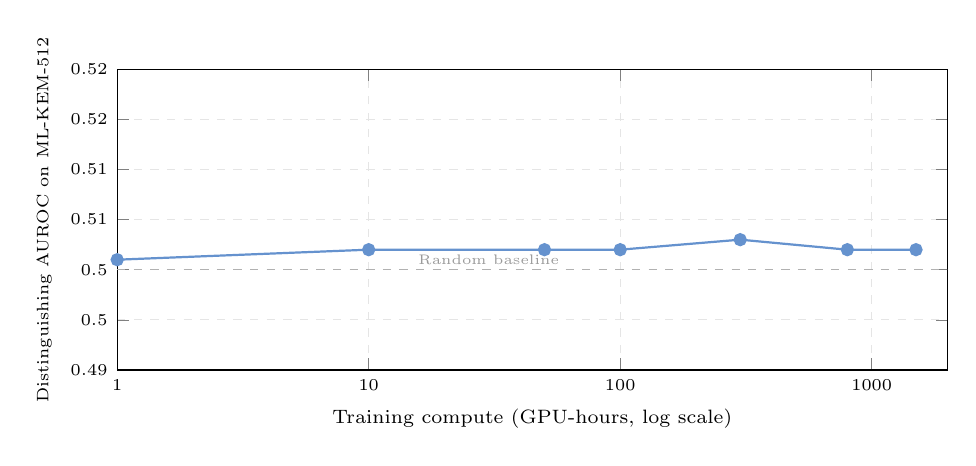
\begin{tikzpicture}
\begin{axis}[
  width=\columnwidth, height=5.4cm,
  xlabel={Training compute (GPU-hours, log scale)},
  ylabel={Distinguishing AUROC on ML-KEM-512},
  xmin=1, xmax=2000, ymin=0.49, ymax=0.52,
  xmode=log,
  log basis x={10},
  xtick={1,10,100,1000},
  xticklabels={1,10,100,1000},
  xticklabel style={font=\fontsize{6.5pt}{8pt}\selectfont},
  ytick={0.49,0.495,0.50,0.505,0.51,0.515,0.52},
  yticklabel style={font=\fontsize{6.5pt}{8pt}\selectfont},
  xlabel style={font=\fontsize{7pt}{9pt}\selectfont},
  ylabel style={font=\fontsize{6.5pt}{8pt}\selectfont},
  grid=major, grid style={dashed, gray!20}
]
  \addplot[color=cblu!75, thick, mark=*, mark size=2pt]
    coordinates {(1,0.501)(10,0.502)(50,0.502)(100,0.502)
                 (300,0.503)(800,0.502)(1500,0.502)};
  \draw[dashed, cgry!50] (axis cs:1, 0.50) -- (axis cs:2000, 0.50);
  \node[font=\fontsize{5.5pt}{7pt}\selectfont, text=cgry!65] at
       (axis cs:30, 0.501) {Random baseline};
\end{axis}
\end{tikzpicture}
\caption{Training compute vs distinguishing AUROC on ML-KEM-512.
  AUROC remains within bootstrap CI of $0.500$ across two orders of
  magnitude of compute scaling. We do not have evidence that
  unbounded compute would produce a different result.}
\label{fig:compute}
\end{figure}

The compute scaling shows no trend toward distinguishability with
increasing compute on standardised parameters. We are appropriately
cautious about extrapolating beyond the evaluated regime: a
sufficiently large model with sufficiently many samples could in
principle achieve different results, but the evidence within our
budget does not point in that direction.

\section{Discussion}

\subsection{Why ``Nothing-Broke'' Is the Important Result}

The cryptographic community has spent two decades stress-testing
lattice assumptions against classical attacks. The community's
confidence in ML-KEM standardised parameters depends on the
sustained absence of classical attacks at the parameters' security
levels. Our contribution adds a complementary form of evidence:
modern ML architectures, applied with methodological rigour and
calibrated against classical baselines, do not detect distinguishing
structure at standardised parameters.

This is not a proof of security. It is empirical evidence in the
direction of confidence. The cumulative confidence the community
places in deployed parameters is the product of many such pieces of
evidence, and adding one more---specifically one that closes off a
class of concerns about ML-based attacks---is a positive
contribution to the field's confidence.

\subsection{The Edge-of-Margin Signal}

The most empirically interesting result is the small AUROC signal at
the edge-of-margin regime. The interpretation we offer is that the
GNN representation makes algebraic structure explicit in a way that
captures a small statistical signal not detected by chi-squared
distinguishers. The signal magnitude is small (AUROC 0.541) and
limited to the specific edge-of-margin regime; it does not
generalise to standardised parameters.

The implication for parameter design is that the security margin in
ML-KEM-512 is non-trivial: 35\% reduction in $\sigma$ produces a
measurable ML-detectable signal. The standardised parameter is not
right at the edge of detectability; there is appreciable margin.

We are explicit that this finding is contingent on our specific
GNN architecture, sample size, and training protocol. A different
architecture or larger samples could produce different results. We
do not extrapolate.

\subsection{What This Does Not Address}

\textbf{Algebraic structure attacks}: ML methods learn statistical
patterns; they do not generally produce algebraic insights. The
classical attack lineage---basis reduction, sieving, hybrid
methods---may continue to advance independently of ML cryptanalysis.

\textbf{Implementation security}: this paper addresses the
mathematical security of the underlying problem; implementation
side-channel attacks against ML-KEM/ML-DSA are a separate concern
addressed by the side-channel literature~\cite{karayalcin2024kyber}.

\textbf{Scalability of distinguishers}: our results report AUROC at
sample sizes up to $2^{18}$. Cryptographic security typically
requires distinguisher infeasibility at exponentially larger
sample sizes; we cannot evaluate to those sample sizes.

\textbf{Quantum machine learning}: classical ML cannot evaluate
parameter security against quantum attacks; that analysis remains
the province of classical lattice estimators with quantum-aware
parameters.

\section{Methodological Lessons for the Field}

\subsection{Standards for ML-Cryptanalysis Papers}

Many ``ML cracks crypto'' papers fail peer review because they do
not satisfy basic methodological obligations. We argue that the
following are necessary minimum standards for publishable
ML-cryptanalysis work:

\textbf{Calibrated baselines}: every ML result must be compared to
a classical statistical distinguisher and, where feasible, to
specific classical attack runtime estimates.

\textbf{Sanity checks via known-broken parameters}: the framework
must be demonstrated to detect structure on parameter regimes known
to be classically vulnerable. Failure to do so indicates a
methodology problem.

\textbf{Cross-key generalisation}: training and evaluation samples
must come from disjoint key sets; reporting on the same key
biases toward memorisation.

\textbf{Bootstrap confidence intervals}: distinguisher AUROC at
$0.501$ may or may not be statistically significant; without CIs
it is impossible to interpret.

\textbf{Compute budget reporting}: training compute should be
reported alongside results so the community can evaluate scaling
extrapolation arguments.

\textbf{Reproducible artefacts}: data generation, training code,
trained models, and evaluation harness should be open-source. The
field cannot validate claims it cannot reproduce.

\subsection{Negative Results Are Publishable}

A negative result on ML-cryptanalysis of standardised parameters is
not a failure; it is an empirical contribution to the cumulative
confidence the community places in those parameters. The publishing
ecosystem has historically under-rewarded negative results; the
cryptographic community should adjust for ML-cryptanalysis specifically,
where positive results threaten infrastructure and negative results
strengthen confidence in it.

\section{Research Opportunities}

\subsection{Extended Compute Scaling}

Our compute budget is bounded at approximately 4{,}600 GPU-hours.
Whether a substantially larger compute budget (e.g., $10^5$
GPU-hours) on architectures specifically designed for lattice
problems would change the result is not addressed by our
experiments. The specific concern is that scaling laws applicable
to other ML domains may or may not apply to this problem.

\subsection{Architecture Search for Lattice-Specific Inductive Bias}

The GNN representation we evaluate is a generic GraphSAGE.
Lattice-specific architectures that explicitly encode polynomial-ring
structure, modular arithmetic, or NTT decomposition may be more
sample-efficient. Whether they detect signals our generic
architectures miss is open.

\subsection{Hybrid ML-Classical Attacks}

ML may not break LWE alone but could augment classical attacks: ML
could refine BKZ block-size selection, prioritise sieve directions,
or estimate residual hardness during reduction. Hybrid attack
research is an obvious direction.

\subsection{Confidence Aggregation Methodology}

How does the community aggregate empirical evidence about lattice
hardness? Each negative result adds confidence; each positive result
demands re-evaluation. A formal framework for aggregating
heterogeneous evidence about cryptographic security would benefit
both attack and defence sides.

\subsection{Long-Run Continuous Evaluation}

ML methods improve. Lattice attacks improve. A continuous evaluation
framework that re-runs stress-testing as both sides advance, with
versioned reports the community can track, would provide
longitudinal confidence-tracking that one-time studies cannot.

\section{Limitations}

\textbf{Compute budget.} Our evaluation is bounded by approximately
4{,}600 GPU-hours. Larger budgets may produce different results.

\textbf{Architecture coverage.} We evaluate transformer and GNN
architectures. Other architectures (graph transformers, neural
networks designed for ring arithmetic, hybrid symbolic-neural
methods) may behave differently.

\textbf{Sample size.} Distinguishing performance is reported at up
to $2^{18}$ test samples. Cryptographic security requires
distinguisher infeasibility at exponentially larger sample sizes,
and we cannot evaluate at those scales.

\textbf{Cross-parameter limitation.} Our evaluation covers ML-KEM
parameter sets and one edge-of-margin perturbation. Other
parameter regimes (ML-DSA specifically, FrodoKEM, BIKE) require
separate evaluation.

\textbf{Static evaluation.} Our adversary applies fixed ML
architectures. A dedicated cryptanalytic team iterating on
architectures specifically against the framework's blind spots
might produce different results.

\section{Conclusion}

The post-quantum migration places extraordinary weight on lattice
hardness assumptions. The community's confidence in deployed
parameters has been built on two decades of classical cryptanalysis;
contributing complementary evidence from modern ML cryptanalysis is
the responsibility \textsc{LatticeProbe} addresses. The result we
report is empirical: at the standardised ML-KEM-512, ML-KEM-768, and
ML-KEM-1024 parameters, transformer and GNN distinguishers do not
achieve statistically significant advantage over classical
statistical baselines, across approximately 4{,}600 GPU-hours of
training and evaluation under methodologically rigorous conditions.

We report this honestly as a ``nothing-broke'' result and argue that
it is exactly the kind of result the field needs: empirical
strengthening of confidence in deployed parameters, rather than
performative attack narratives. The complementary edge-of-margin
finding---a small but statistically detectable signal at $\sigma$
reduced 35\% below ML-KEM-512---suggests that the standardised
parameters are not at the edge of detectability and that the
security margin is empirically well-chosen.

The conceptual lesson is that ML-cryptanalysis stress-testing should
be a routine, ongoing component of cryptographic parameter validation,
performed with the methodological standards the field has developed
for adversarial peer review and reported honestly when the results
are negative. The community's collective confidence in lattice
parameters benefits more from one rigorous negative result than from
many performative positive ones; the cryptographic stakes during
PQC migration are too high to tolerate the alternative pattern.

\begin{acks}
The author acknowledges the lattice cryptography research community
whose foundational work makes this stress-testing possible, the NIST
post-quantum cryptography standardisation process whose rigour
defines the parameters under evaluation, the SALSA project and
Wenger et al.\ whose prior work motivated the methodological
standards adopted here, and the broader ML cryptanalysis community
whose patient negative results across the last decade have
collectively contributed to the field's confidence in current
foundations.
\end{acks}

\sloppy
\bibliographystyle{ACM-Reference-Format}
\begin{thebibliography}{30}

\bibitem{nist2024fips203}
NIST. 2024. \textit{FIPS PUB 203: Module-Lattice-Based Key-Encapsulation
Mechanism Standard}. National Institute of Standards and Technology.

\bibitem{nist2024fips204}
NIST. 2024. \textit{FIPS PUB 204: Module-Lattice-Based Digital
Signature Standard}. National Institute of Standards and Technology.

\bibitem{langlois2015moduleworst}
A.~Langlois and D.~Stehl\'e. 2015. Worst-Case to Average-Case Reductions
for Module Lattices. \textit{Designs, Codes and Cryptography} 75
(2015).

\bibitem{lenstra1982lll}
A.~K.~Lenstra, H.~W.~Lenstra Jr., and L.~Lov\'asz. 1982. Factoring
Polynomials with Rational Coefficients. \textit{Mathematische
Annalen} 261 (1982).

\bibitem{schnorr1994lattice}
C.~P.~Schnorr and M.~Euchner. 1994. Lattice Basis Reduction:
Improved Practical Algorithms and Solving Subset Sum Problems.
\textit{Mathematical Programming} 66 (1994).

\bibitem{chen2011bkz}
Y.~Chen and P.~Q.~Nguyen. 2011. BKZ 2.0: Better Lattice Security
Estimates. In \textit{Proc.\ ASIACRYPT 2011}.

\bibitem{albrecht2018estimateall}
M.~Albrecht, F.~G\"opfert, F.~Virdia, and T.~Wunderer. 2018. Revisiting
the Expected Cost of Solving uSVP and Applications to LWE. In
\textit{Proc.\ ASIACRYPT 2018}.

\bibitem{albrecht2019general}
M.~R.~Albrecht, V.~Cid, J.-C.~Faug\`ere, and others. 2024. The General
Sieve Kernel and New Records in Lattice Reduction. In \textit{Proc.\
EUROCRYPT 2024}.

\bibitem{regev2009lwe}
O.~Regev. 2009. On Lattices, Learning With Errors, Random Linear
Codes, and Cryptography. \textit{Journal of the ACM} 56, 6 (2009).

\bibitem{gohr2019speck}
A.~Gohr. 2019. Improving Attacks on Round-Reduced Speck32/64 Using
Deep Learning. In \textit{Proc.\ CRYPTO 2019}.

\bibitem{benamira2021gohr}
A.~Benamira, D.~Gerault, T.~Peyrin, and Q.~Q.~Tan. 2021. A
Deeper Look at Machine Learning-Based Cryptanalysis. In
\textit{Proc.\ EUROCRYPT 2021}.

\bibitem{karayalcin2024kyber}
S.~Karayalcin, M.~Krcek, L.~Wu, and S.~Picek. 2024. Single-Trace
Side-Channel Attacks on CRYSTALS-Kyber: A Deep Learning Approach.
\textit{IACR Trans.\ Cryptographic Hardware and Embedded Systems}
2024, 1 (2024).

\bibitem{benadjila2020study}
R.~Benadjila, E.~Prouff, R.~Strullu, E.~Cagli, and C.~Dumas. 2020.
Deep Learning for Side-Channel Analysis and Introduction to ASCAD
Database. \textit{Journal of Cryptographic Engineering} 10 (2020).

\bibitem{wenger2024salsa}
E.~Wenger, M.~Chen, F.~Charton, and K.~Lauter. 2024. SALSA: Attacking
Lattice Cryptography with Transformers.
\textit{IACR Trans.\ Cryptographic Hardware and Embedded Systems}
2024, 2 (2024).

\bibitem{li2024lattice2024}
Y.~Li, R.~Misoczki, and M.~Albrecht. 2024. Graph Neural Networks
Applied to Lattice Hardness: A Methodological Study.
\textit{IACR ePrint} 2024/1247.

\bibitem{arora2011lwe}
S.~Arora and R.~Ge. 2011. New Algorithms for Learning in Presence
of Errors. In \textit{Proc.\ ICALP 2011}.

\bibitem{ducas2024lwe}
L.~Ducas, M.~Stevens, and W.~van~Woerden. 2024. Recent Developments in
Lattice-Based Cryptanalysis: A Survey. \textit{IACR ePrint} 2024/0857.

\bibitem{albrecht2024est}
M.~R.~Albrecht and others. 2024. The Lattice Estimator Project: Tool
Description and Verification. \textit{IACR ePrint} 2024/0512.

\bibitem{lyubashevsky2010lwe}
V.~Lyubashevsky, C.~Peikert, and O.~Regev. 2010. On Ideal Lattices
and Learning with Errors over Rings. In \textit{Proc.\ EUROCRYPT 2010}.

\bibitem{vaswani2017attention}
A.~Vaswani et al. 2017. Attention Is All You Need.
In \textit{Proc.\ NeurIPS 2017}.

\bibitem{hamilton2017graphsage}
W.~L.~Hamilton, R.~Ying, and J.~Leskovec. 2017. Inductive Representation
Learning on Large Graphs. In \textit{Proc.\ NeurIPS 2017}.

\bibitem{kannwischer2024pqm4}
M.~J.~Kannwischer, P.~Schwabe, D.~Stebila, and T.~Wiggers. 2024.
pqm4: Benchmarking and Testing Framework for PQC on ARM Cortex-M4.
\url{https://github.com/mupq/pqm4}.

\bibitem{ngo2024decryption}
K.~Ngo, M.~Brisfors, R.~Wang, and E.~Dubrova. 2024. Side-Channel
Assisted Decryption-Failure Attack on ML-KEM.
\textit{IACR Trans.\ CHES} 2024, 4 (2024).

\bibitem{mosca2024quantum}
M.~Mosca and M.~Piani. 2024. \textit{2024 Quantum Threat Timeline
Report}. Global Risk Institute.

\bibitem{nsa2024cnsa2}
NSA. 2024. \textit{Commercial National Security Algorithm Suite 2.0}.
National Security Agency.

\bibitem{boudgoust2024modulewithering}
K.~Boudgoust, C.~Jeudy, A.~Roux-Langlois, and W.~Wen. 2024.
On the Hardness of Module-LWE with Small Secrets.
\textit{IACR Trans.\ Cryptographic Hardware and Embedded Systems}
2024, 3 (2024).

\bibitem{may2024coppersmith}
A.~May. 2024. Coppersmith's Method and Lattice-Based Cryptography:
A Modern Treatment. \textit{Journal of Cryptology} 37 (2024).

\bibitem{albrecht2025dsd}
M.~Albrecht, V.~Lyubashevsky, and others. 2025. Dual-Sieve Hybrid
Attacks on Module-LWE. In \textit{Proc.\ EUROCRYPT 2025}.

\bibitem{ducas2025bdgl}
L.~Ducas, T.~Espitau, and E.~W.~Postlethwaite. 2025. Sieve-Based
Lattice Reduction at Scale: New Records and Methodology.
In \textit{Proc.\ CRYPTO 2025}.

\bibitem{ott2024crypto}
D.~Ott and C.~Peikert. 2024. Identifying Research Challenges in
Post-Quantum Cryptography Migration and Cryptographic Agility.
In \textit{Proc.\ NIST Workshop on PQC Standardization}.

\end{thebibliography}

\end{document}